\chapter{The LHC and The CMS Experiment}

\section{The LHC}

The Large Hadron Collider (LHC) is the largest and most powerful hadron accelerator and collider. The LHC was installed in an existing 26.7 km tunnel that was constructed for LEP machine between 1984 and 1989. The tunnel of LHC has 8 straight sections and 8 arcs, and locates between 45m and 170m below the surface. The LHC hosts 4 experiments currently: CMS (Point 5), ATLAS (Point 1), ALICE (Point 2) and LHCb (Point 8). The LHC can accelerate the proton beam to 7TeV (running on 6.5TeV during the LHC run2).

However, the LHC is not the only accelerator that boosts the proton to such a high energy. The LHC is the last and biggest accelerator in the whole chain. A simplified injection chain can be described by Fig.~\ref{fig:c3lhclpsspslhc}. Physicists inject hydrogen gas into a metal cylinder, and then put a strong electrical field to strip the electron from hydrogen to obtain proton beam. The protons will be accelerated to 90keV with a DC voltage power supply. Then a Radio Frequency Quadrupole (QRF) will focus and boost the protons beam to 750keV. After that, the proton beam will be injected to a linear accelerator (LINAC2) and accelerated to 50MeV. The current LHC uses the LINAC2 as the source of protons. The LINAC2 will be replaced by LINAC4 with negative hydrogen ion source, higher beam intensity and energy (160MeV) in 2019-2020. 

\begin{figure}[htbp]
 \begin{center}
  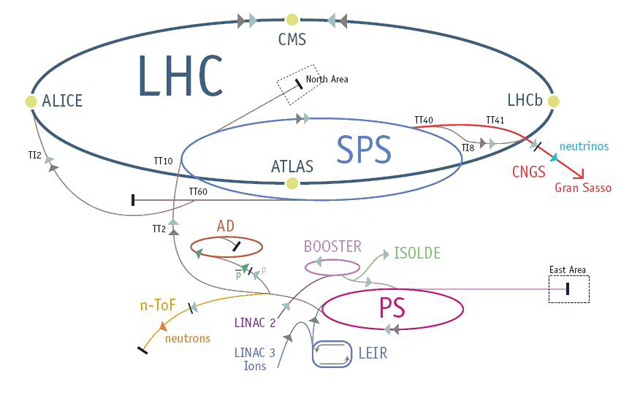
\includegraphics[width=0.8\textwidth]{figures/c3/c3_lhc_lpsspslhc.jpg}
 \end{center}
 \caption{The LHC full injection chain}
 \label{fig:c3lhclpsspslhc}
\end{figure}

The proton beam will be boosted to 6.5TeV with four circular accelerators from the linear accelerator. The first one in the chain is the proton synchrotron booster (PSB, Fig.~\ref{fig:c3lhcpsb}), a four-ring slow-cycling synchrotron. The PSB is inserted in between the LINAC and proton synchrotron in 1972 to increase the beam intensity. The PSB will bring the proton energy up to 1.4GeV in 530ms and then inject the beam to the proton synchrotron (PS). The proton will be accelerated to 25GeV inside the PS. PS is also responsible to form the standard injection beam for the LHC. Then, the super proton synchrotron (SPS) will take over the beam from PS and boost it to 450GeV in 4.3 seconds. And finally, the protons arrive to the LHC tunnel and obtain the 6.5TeV energy in 25min during beam ramp up. 

\begin{figure}[htbp]
 \begin{center}
  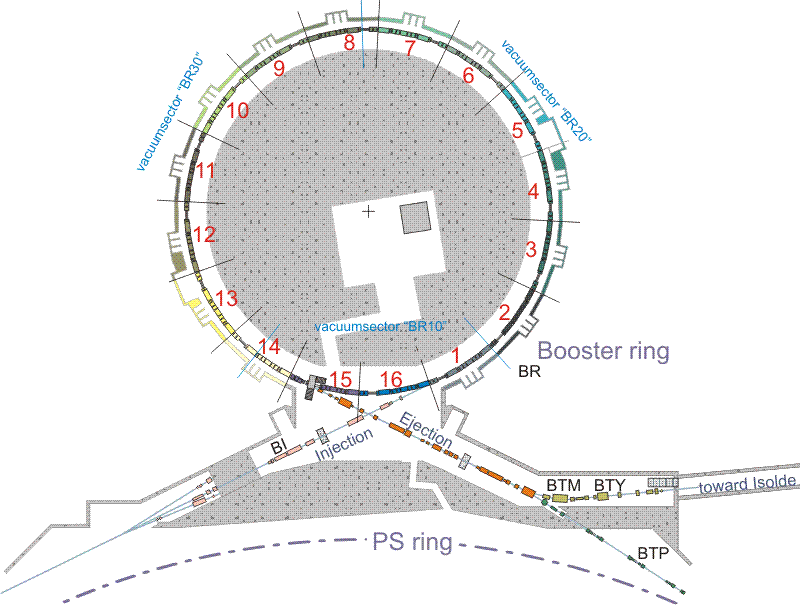
\includegraphics[width=0.8\textwidth]{figures/c3/c3_lhc_psb.png}
 \end{center}
 \caption{The PS layout}
 \label{fig:c3lhcpsb}
\end{figure}

We can have a simple calculation to obtain how long it takes from the LINAC2 to 450GeV SPS: 0.53+1.025+4.3=5.86 seconds. However, we also split one fill of the beam into several bunches and batches with certain time spacing to obtain a desired luminosity. Therefore, we have latency for different batch and the 5.86 seconds is just a lower limit for pre-LHC acceleration time. 

The fill scheme before the LHC is relatively stable in the machine in the proton physics mode. The injection beam from PSB to PS contains 2 batches, 4 bunches for the first batch and 2 for the second. The first will take an additional 1200ms to be delivered. The proton beam will go through one triple split and two double splits. A 72 bunches beam will be formed after the splitting and delivered to SPS in a group of 4 72-bunch batches. The latencies are 10.8 seconds for the first batch, 7.2 for the second, 3.6 for the third and 0 for the fourth. Therefore, the maximum time from the LINAC2 to 450GeV SPS is 0.53+1.2+1.025+10.8+4.3=17.86 seconds. 

The LHC fill scheme can be different for various purposes. One of the common fill scheme in the operation is 2808 bunches per LHC ring. The fill scheme can be described by the Fig.~\ref{fig:c3lhcfillscheme}. The SPS will have 12 injections to the LHC. The number of 72-bunch batches are in pattern of 234 334 334 334. We will have different luminosities for different fill schemes. In the detector operation, it is important to know the fill scheme and expected luminosity in advance to design the trigger menu in different bias level. 

\begin{figure}[htbp]
 \begin{center}
  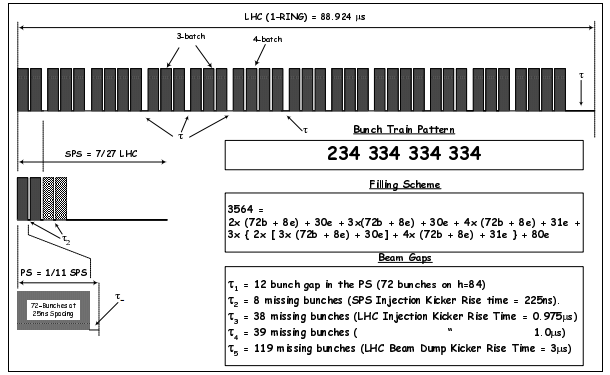
\includegraphics[width=0.8\textwidth]{figures/c3/c3_lhc_fillscheme.png}
 \end{center}
 \caption{Schematic of the Bunch Disposition around an LHC Ring for the 25ns Filling Scheme}
 \label{fig:c3lhcfillscheme}
\end{figure}

\subsection{LHC: Machine layout and Performance}

The LHC is a near-circle ring with 8 arcs and 8 straight sections (Fig.~\ref{fig:c3lhclayout}). Each straight section is around 528m long and can host detector system or beam related insertions. The two high luminosity experiments are located at opposite straight sections: ATLAS at point 1 and CMS at point 5. The ALICE experiment and the beam1 injection system are located at point 2, while the LHCb and beam2 injection system are at point 8. 

\begin{figure}[htbp]
 \begin{center}
  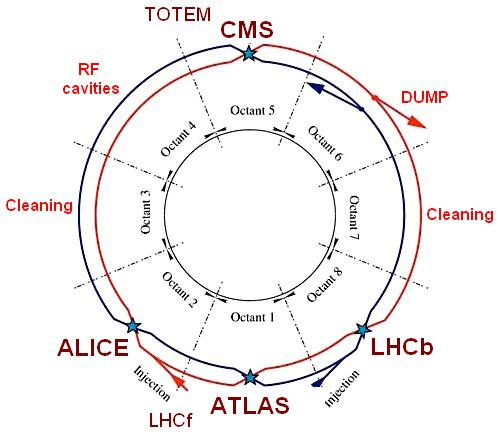
\includegraphics[width=0.8\textwidth]{figures/c3/c3_lhc_latticelayout.jpg}
 \end{center}
 \caption{The LHC layout}
 \label{fig:c3lhclayout}
\end{figure}

Two collimation systems are located at point 3 and point 7 respectively. The collimation system can protect the machine against unavoidable regular or irregular beam loss. The collimator at point 3 is designed to clean beam transverse momentum dispersion and the one at point 7 is for beam betatron emission. The materials of the collimators are required to be extremely radiation hard because they are installed in the most active region of the LHC. 

The beam dump insertion is sat in the point 6. There are three steps to dump the beam: extraction, dilution and absorption. The magnet kicker will be turned on in 3000ns, which is the gap reserved for each orbit cycling. Then the beam will be kicked off by a 0.27 mrad angle. The extracted beam will be swept in a quasi-circular figure by two sets of deflecting dilution kickers. Finally, a 7m long segmented carbon cylinder will absorb the beam.

The point 4 is the only straight section that contains the acceleration systems. Two radio frequency systems are installed for beam1 and beam2 respectively. 

One of the aims of the LHC is the reveal the physics beyond the standard model. The exploration of the rate events in the LHC requires both high beam energies and high beam intensities. The energy of the beam is limited by the machine geometry. The luminosity of the machine can be described by the Eq.~\ref{eq:c3lhclumi} with the Gaussian beam distribution. The $N_{b}$ is the number of particles per bunch and $n_{b}$ is the number of bunches per beam. This indicates we can increase the luminosity with the optimization of fill scheme. The $f_{rev}$ is the revolution frequency, $gamma_{r}$ is the relativistic gamma factor, $\varepsilon_{n}$ is the normalized beam emittance and $\beta *$ is the impact parameter at the collision point. The F is the geometric luminosity reduction factor due to the crossing angle at the interaction point. 

\begin{equation}
 L = \frac{N^{2}_{b}n_{b}f_{rev}\gamma_{r}}{4\pi \varepsilon_{n}\beta *}F \;
 \label{eq:c3lhclumi}
\end{equation}

The definition of F is in the Eq.~\ref{eq:c3lhcgeof}. The $\theta_{c}$ is the full crossing angle at the interaction point, the $\sigma_{z}$ is the RMS bunch length and $\sigma *$ is the transverse RMS beam size at the interaction point. The LHC experts are trying to reduce the crossing angle from 370 to 280 mrad, which increase the peak luminosity by 15 percents. 
\begin{equation}
 F = (1+\frac{\theta_{c}\sigma_{z}}{2\sigma *})^{-1/2} \;
 \label{eq:c3lhcgeof}
\end{equation}

In the CMS and ATLAS experiments, the designed peak luminosity at the collision point is approximately $10^{34}cm^{-2}s^{-1}$. The LHC has achieved this goal in 2016 and try to increase the luminosity with optimizations.

\subsection{LHC: From operation point of view}

The LHC is an extremely complex machine and it is almost impossible to grasp every details. However, the LHC provides a summary of status for the operational activities, which are very useful in the detector operation.

\subsubsection{Acclerator Mode}

The accelerator mode provides a summary status of the LHC machine. All the accelerator modes are listed in the Table~\ref{tab:c3lhcaccmode}. The accelerator modes can be categorized into two groups by the existence of the beam. For example, ACCESS mode means the LHC or at least one of the detector system need to investigate their issue in the cavern. The beam must be dumped during this access period. Another example is the BEAM SETUP mode, which means the beam under preparation. The beam mode may change during this accelerator mode. The beam modes are described in the following section. The detector system (e.g. CMS) will make daily operational decision according to the accelerator modes and beam modes provided by the LHC.

\begin{table}[htbp]
\fontsize{10 pt}{1.2 em}
\selectfont
\begin{centering}
\caption{\label{tab:c3lhcaccmode} Acclerator Mode}
\hspace*{-4ex}
\begin{tabular}{|c|c|c|}
\hline
 Mode Name &  Description & Beam exist \\
\hline
 SHUTDOWN & \specialcell{Machine not running} & NO BEAM \\
\hline
 COOLDOWN & \specialcell{Machine comes back from shutdown,\\ cryogenics related activities going on} & NO BEAM \\
\hline
 MACHINE CHECKOUT & \specialcell{Checking out LHC subsystems} & NO BEAM \\
\hline
 ACCESS & \specialcell{Access going on} & NO BEAM \\
\hline
 MACHINE TEST & \specialcell{Operation tests without beam} & NO BEAM \\
\hline
 CALIBRATION & \specialcell{Power converter calibration} & NO BEAM \\
\hline
 WARM-UP & \specialcell{Sectors warm up for repair} & NO BEAM \\
\hline
 RECOVERY & \specialcell{Quench recovery} & NO BEAM \\
\hline
 SECTOR DEPENDENT & \specialcell{Sector activities going on} & NO BEAM \\
\hline
 BEAM SETUP & \specialcell{Machine setup with 1 or 2 beams,\\ usually a signal of next physics fill when taking data} & BEAM \\
\hline
 PROTON PHYSICS & \specialcell{Beam on for proton physics} & BEAM \\
\hline
 ION PHYSICS & \specialcell{Beam on for ion physics} & BEAM \\
\hline
 TOTEM PHYSICS & \specialcell{Beam on for TOTEM physics} & BEAM \\
\hline
 MACHINE DEVELOPMETN & \specialcell{Beam on machine development} & BEAM \\
\hline
\end{tabular}
\par\end{centering}
\end{table}

\subsubsection{Beam Mode}
The beam modes are showed in the Table~\ref{tab:c3lhcbeammode}. The beam modes describe standard injection procedures and accidental abort issues of the 2 beams in the LHC. A standard successful injection for physics should have the following beam modes in chain during BEAM SETUP accelerator mode:

\begin{itemize}
\item BEAM SETUP: The SPS is injecting beam bunches into the transfer line. The beam is not circulating in the LHC yet.
\item INJECTION PROBE BEAM: A test beam with relatively smaller intensity is injected into the LHC from the transfer line. Although we have machine protection system to shield the LHC from the beam, we still need to make sure the system is safe for circulating. A less dense beam is a proper test for this aim.
\item INJECTION SETUP BEAM and INJECTION PHYSICS BEAM: The LHC will measure the beam properties. Then a full intensity beam will be injected for physics data taking.
\item PRERAMP and RAMP: The LHC ramp the beam energy up with the radio frequency system.
\item FLAT TOP and SQUEEZE: The LHC will check the system. Then the beam will be focused to reduce the impact parameter.
\item ADJUST and STABLE BEAM: The LHC will adjust beam before collision. Then we can begin to enjoy the data rain.
\end{itemize}

\begin{table}[htbp]
\fontsize{10 pt}{1.2 em}
\selectfont
\begin{centering}
\caption{\label{tab:c3lhcbeammode} Beam Mode}
\hspace*{-4ex}
\begin{tabular}{|c|c|c|}
\hline
 Mode Name &  Description \\
\hline
 SETUP & \specialcell{Beam in transferline, but not in the ring} \\
\hline
 ABORT & \specialcell{Recovery mode following beam drop} \\
\hline
 INJECTION PROBE BEAM & \specialcell{Ring is injected with test beam for safe circulating} \\
\hline
 INJECTION SETUP BEAM & \specialcell{Beam measurement going on after probe beam\\ but before injection physics beam} \\
\hline
 INJECTION PHYSICS BEAM & \specialcell{Beam for physics is injected in the ring} \\
\hline
 PRERAMP & \specialcell{Injection done, prepare for ramp} \\
\hline
 RAMP & \specialcell{Ramp up the beam energy} \\
\hline
 FLAT TOP & \specialcell{Ramp done, pre-squeeze checks} \\
\hline
 SQUEEZE & \specialcell{Squeezing the beam size} \\
\hline
 ADJUST & \specialcell{Preparing for collision or after collision} \\
\hline
 STABLE BEAMS & \specialcell{Stable collision, detector should taking data} \\
\hline
 UNSTABLE BEAMS & \specialcell{Unstable beam because of sudden beam degradation} \\
\hline
 BEAM DUMP WARNING & \specialcell{Beam dump warning in case of emergency beam dump} \\
\hline
 BEAM DUMP & \specialcell{End of physics collision} \\
\hline
 RAMP DOWN & \specialcell{Ramp down beam energy after programmed dump} \\
\hline
 CYCLING & \specialcell{Pre-cycle before injection\\ following access, recovery, etc} \\
\hline
 NO BEAM  & \specialcell{No beam exist} \\
\hline
\end{tabular}
\par\end{centering}
\end{table}

The beams modes are used to estimate the time remain before next collision. For example, the CMS system requires all the subsystem to be ready for data taking when the LHC declare the injection physics beam. Some of the subsystems need to do the alignment or calibration during this period. The time estimation from the LHC beam status is important for a smooth data taking.

\section{The CMS Experiment}

The CMS Experiment is a particle physics experiment based on CMS detector system on the LHC. It contains with CMS detector system and event reconstruction, supported by the detector operation team, computing/storage department and software fraction.

\subsection{CMS Detector System}

The Compact Muon Solenoid (CMS) is one of the general-purpose detection system on the LHC. To fullfill the "general-purpose", the CMS is designed as a combo of several subsystems: Sillicon Pixels and Strips for tracking information, Electromagnetic and Hadron Calorimeters for "light" particle energy deposition and drift tubes and cathode strip/resisstive plate chambers for muon details. The locations of these subdectors in the CMS are not random: The sillicon tracking subsystems are located on the inner CMS, closest to the collision point, and the calorimeter subsystems after the sillicon subdetectors, because of its destructive detection nature; Finally the muon system in the outer layer to capture our heavy object which go through the calorimeter subsystems. To obtain the high performance, the CMS is immersed in a 4-T field, which is powered by a superconducting solenoid("S" in CMS). The magnet components have a major contribution on the CMS total weight: 12500 tones out of 14000. However, comparing with its heavy weight, the size of the CMC system is relatively small: only 5000 $m^{3}$. Then the given name "Compact" is imposed in front of "Muon Solenoid" since its density near to 3000 $kg/m^{3}$.

\subsubsection{Inner Tracking system}

As described in the name - - - inner tracking system, there are two main features for this CMS sub-detector: the closest sub-detector to the LHC beam and tracks reconstruction. The main challenge is a consequence of the first feature: the inner tracking systems have to be radiation hard during the expected lifetime of 10 years (LHC run1+run2+run3). More over, since the LHC have high intensity and small bunch crossing (25ns), we also need the inner tracking systems to have a fine granularity and fast response. The silicon based technology detector is the best option to satisfy all these requirements. On the other hand, the second feature actually comes from the physics requirement. We need to reconstruct the tracks of charged particles and secondary vertices in the event from the three dimensional hits. The tracks information are not only used in the charged particle reconstruction, but also applied in the particle flow algorithm as a base of all physics objects in CMS collaboration. The secondary vertices are also important in the heavy flavor objects reconstruction, and new physics search of long-lived particles. 

As a result of budget-performance balance, the CMS inner tracking systems are designed as a combination of two sub-systems: the silicon pixel and the silicon strip. A schematic drawing of the CMS tracking system is shown in the Fig.~\ref{fig:c3cms2dtracker}. More details will be described in the following sections. 

\begin{figure}[htbp]
 \begin{center}
  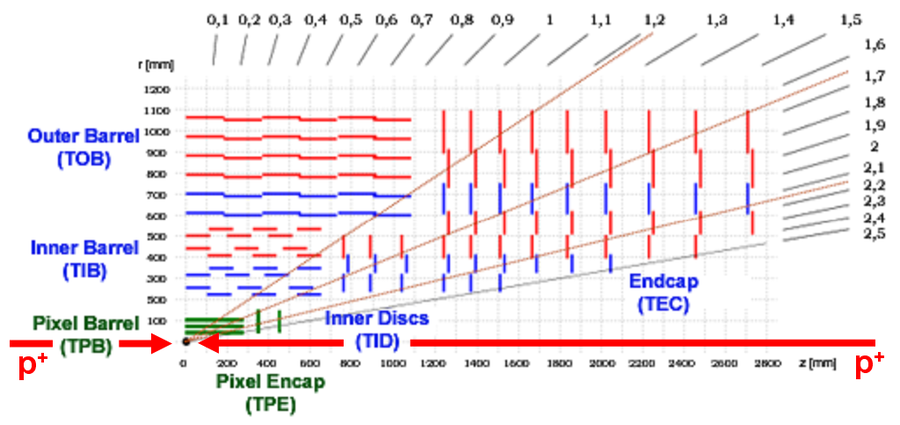
\includegraphics[width=0.8\textwidth]{figures/c3/c3_cms_2dtracker.png}
 \end{center}
 \caption{Two dimensional CMS inner tracking system layout, phrase 0}
 \label{fig:c3cms2dtracker}
\end{figure}

\paragraph{Silicon Pixels}

The pixel system is the part of inner tracking system that closest to the collision point. It provides a precise measurement of the tracking points; therefore contribute a lot for the secondary vertex reconstruction. The pixel cells are distributed with size of 100 num*150 num in three-dimensional space, which allow a 3D reconstruction method for the secondary vertex offline. Readout chips bump bonded to the sensor read out the signals from pixel cells. Then the signal will be delivered to the frondend driver through the analog chain once we receive a positive bit from L1 trigger.

The phrase 0 pixel detector contains three barrel layers (BPix) and two endcap disks (FPix), which covers a pseudo rapidity range $-2.5<\eta<2.5$. In phrase 1 upgrade, to suffer from the radiation damage, we replaced all layers and disks with new ones, and added one layer in the barrel region, one disk in the endcap region.

One special design of the pixel detector is the blade that module mounted are rotated by 20 degrees in a turbine geometry. Such an arrangement enhanced the charge sharing effects between the nearby pixels. The space resolution can be improved to 15num by the using the "charge sharing" effect in pixels. CMS take advantage of this effect with the analog readout of the collected charges by readout pixels in-group with readout chips. 

\paragraph{Silicon Strips}

The particles pass through ten layers of silicon strip detectors after the pixel. The strip detector provides a complete charged track together with the pixel detector. The silicon strip tracker is composed of 15148 detector modules. Each module carries either one 320 num or two 500 num silicon sensors from a total of 24244 sensors. The charges that come out of sensor will be amplified, shaped and stored by a custom integrated circuit. Once received a positive L1 trigger decision, the analog signal will be multiplexed and transmitted via optical link to the front end driver, then digitalized. 

The inner strip detector contains 4 barrel layers (TIB) and 3 disks (TID) support for each side. The outer strip detector has 6 barrel layers (TOB, 2 double-sided, 4 single-sided) and the endcap strip has 9 disks (TEC) on each side.

The online alignment system for the strip detector is necessary with the complicate structure and resolution requirement in physics performance. The laser alignment system is designed and built in to monitor the stability and the alignment of the strip detector mechanical structure. The infrared laser light will be delivered directly to the sensor on the 434 silicon modules (3\%) to trigger a signal pulse. The alignment data can be taken during commission, inter-fill period and also in the orbit gap when we have stable beam. Since the pixel will be aligned with strip through the reconstructed tracks, the strip alignment is the only online and direct alignment for the whole inner tracking system. 


\subsubsection{Calorimeters}
\paragraph{Electromagnetic Calorimeter}
The CMS electromagnetic calorimeter (ECAL) is a hermetic homogeneous calorimeter made of by lead tungstate (PbWO4) crystals. The lead tungstate is an appropriate choice for CMS ECAL because the crystal is both radiations hard in LHC environment and response rapid (same level as the LHC bunch crossing). 61200 lead tungstate crystals are installed in the ECAL barrel region while 7324 for endcap. The lead tungstate will emit 80\% of the light in 25 ns once the electron (or photon) hits on the crystal.

Then we need a photon detector to collect the light yield from crystals. As the request we have for the crystal, we also need the photon detector to be both radiation tolerant and fast. To satisfy the requirement, the avalanche photodiodes (APD) are installed in barrel while the vacuum phototriodes in the endcap. All the photon detectors have been tested in the harsh environment (high radiation plus 4T magnet field) before actually installed. The light yield from the crystal is weak, so we also need to amplify them with photomultiplier. The multi gain pre-amplifiers (MGPA), an ASIC specifically designed for ECAL, are installed to reshape and amplify the signal from photon detectors.

Then the amplified electrons will be integrated and digitized by the on-detector electronics and then pass to the central data acquisition from the off-detector electronics. The electronics, especially for the off-detector electronics, the ECAL is very similar with the HCAL (hadron calorimeter) counterpart, I will show more details in the next section since I am majorly working for HCAL in my PhD period. 

The last thing need to mention is the preshower system for ECAL endcap. We have high-energy neutral pion in endcap region, and the prompt photons from the high-energy neutral pion can be an issue in the physics analysis since they are almost collinear. The major purpose of the preshower detector is to trigger the electromagnetic shower with high spatial resolution before ECAL endcap. As a result, the almost collinear photons can be distinguished by the ECAL reconstruction hits occupancy. 

\paragraph{Hadron Calorimeter}

The CMS HCAL is sets of detectors that measure the energy of hadronic particles consist of quarks and gluons. It contains four parts: Hadron Barrel (HB), Hadron Endcap (HE), Hadron Outer (HO) and Hadron Forward (HF). The overall geometry scheme plot is showed in Fig.~\ref{fig:c3cms2dhcal}. The CMS HCAL is a sampling calorimeter with brass absorber for shower trigger and scintillator for energy measurement. We take advantage from the dense absorber to fit the HCAL in the limited space inside the solenoid (Except for HO). However, we also suffer with the relatively big fluctuation in energy deposit due to the invisible energy loss in the absorber and uncompensated design of the calorimeter. The following paragraphs will have more description for HBHE, HO and HF.

\begin{figure}[htbp]
 \begin{center}
  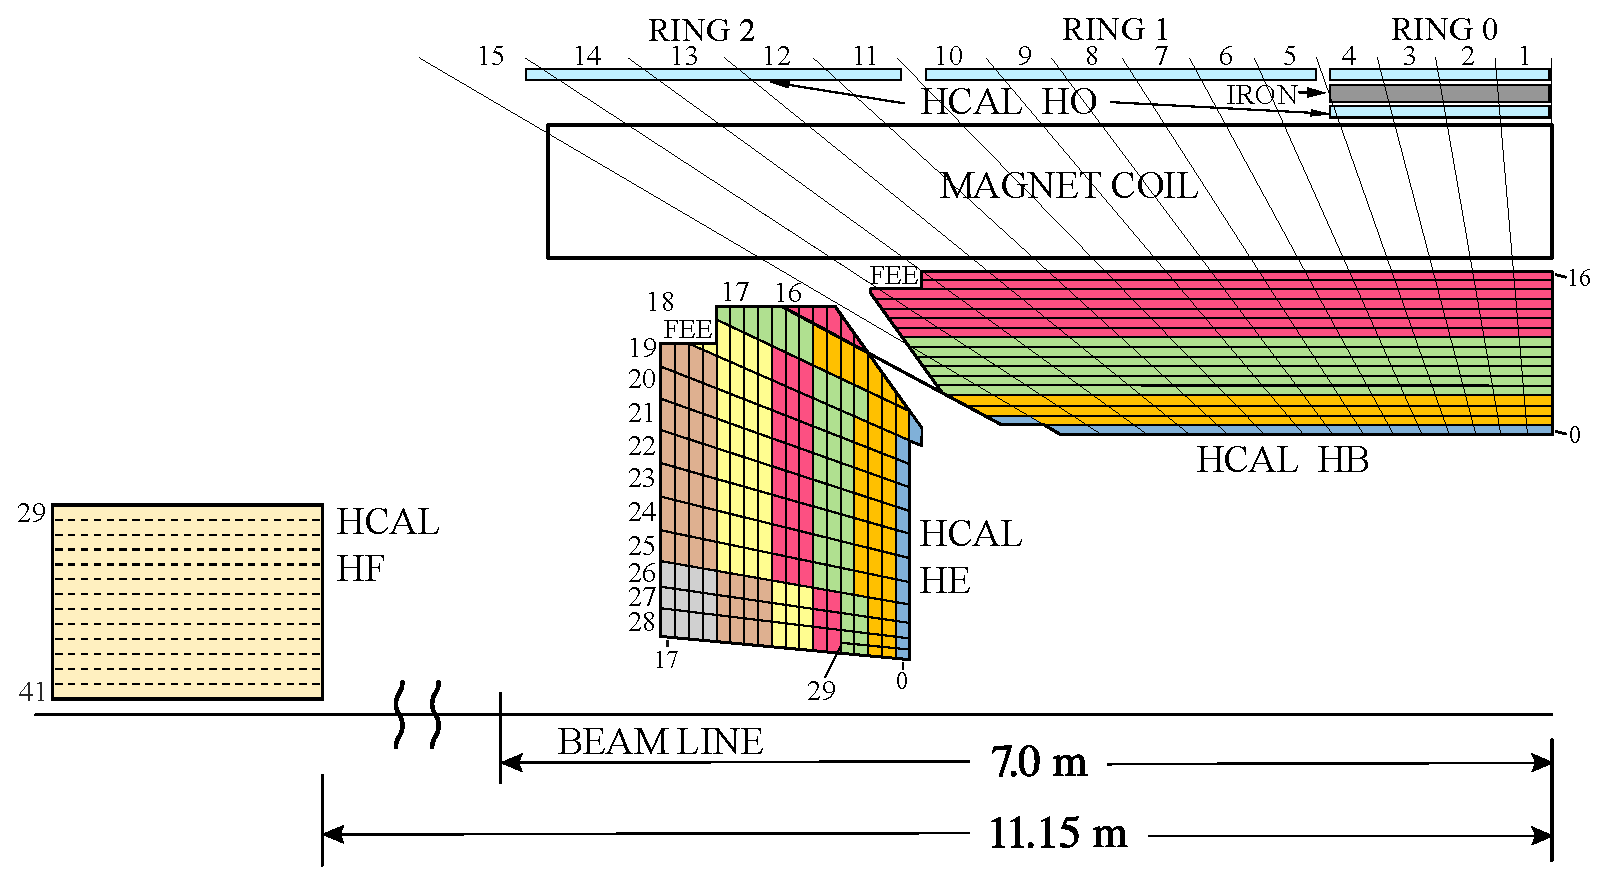
\includegraphics[width=0.8\textwidth]{figures/c3/c3_cms_2dhcal.pdf}
 \end{center}
 \caption{Phrase 1 HCAL tower segmentation in the r,z plane}
 \label{fig:c3cms2dhcal}
\end{figure}

The HB and HE are major parts of the HCAL. As I mentioned before, they are typical sampling calorimeters with brass from Russia navel bullet and scintillator for ~ 70000 tiles. The lights from the scintillators is collected and amplified by hybrid photodiodes (HPDs) for phrase 0 HCAL. The HPDs will be replaced with Silicon photomultipliers (SiPMs) since the SiPMs are less noisy and more stable under heavy radiated area. 

After the photon detectors, the analog signal will be delivered to the FrontEnd electronics. The charge pulse will be integrated and digitized on the charge integrate encoder (QIE). In the phrase 1 upgrade, we will replace the QIE8 with QIE11 for all frontend readout modules in HE. The QIE11 have a much better time resolution in level of 0.5ns. 

After the FrontEnd, the digitalized signal will be delivered from the commission cavern to the service cavern through a long bonded fibers bundle. The backend electronics located in the service cavern will receive those signals, generate the trigger primitives and deliver the signals to the central DAQ link. The HCAL backend have been upgraded from VME to uTCA on HBHE since 2015-2016 YETS. 

However, due to the limitation on the "compact" cavern, the EB (ECAL barrel) and HB cannot provide sufficient containment for the hadron showers. The HO is inserted just between the solenoid and muon system to ensure the adequate sampling depth in the barrel region. The solenoid coil is used as the absorber for HO to measure the shower deposit after HB. 

The HO instruments is same as the phrase 0 HBHE, except for the photon detectors. The HO team has replaced the HPDs with the SiPMs since the LHC long shut down 1. The SiPMs have been proved super reliable in the current operation except a small leakage current drift monitoring issue at the beginning of LHC run 2. 

The last component of HCAL is the Forward calorimeter. The calorimeter material is severely challenged by the extremely high radiation environment. Therefore, the quartz fibers are used as the active medium for forward calorimeter. Upon shower comes, the Cherenkov light will be emitted in the quartz fiber and transported to the photomultiplier tubers (PMT). The HF also provides input to the CMS luminosity measurement. 

To sum up, we have four partitions in HCAL: HB, HE, HO and HF. We have 9216 readout channels for HB, 6912 for HE, 2376 for HO and 3456 for HF in the HCAL phrase 1 scheme. The backend electronics coordinates will be compressed into the RAW event data after the event builder in HLT. On one hand, the offline reconstruction software and online data quality monitor need to know the detector geometry coordinators to show the digitalized output in the physical space. We need to build a database object to map the backend coordinates and detector coordinates. On the other hand, the backend electronics are not connected directly to the HCAL tiles: we still have photomultiplier and frontend electronics in between. And HCAL has several different upgrade projects for different parts on different sub detectors during the LHC run2. Therefore, we need a dynamic map, which reflects the real connections among all HCAL components. This map is called HCAL Logical Map. The logical will start with frontend coordinates, map upwards to photomultipliers, then detector tiles, downwards to the backend coordinates then trigger primitive channels. We avoid re-designing everything after the each upgrade with this dynamic structure of map. 

To build a robust HCAL Logical map, we need inputs from experts in different fields. For example, we need to follow a special symmetric design in the frontend to backend optical patch. This symmetry is highly dependent on the firmware design. Although nowadays FPGA can be programmed with less restrict, we still need to keep the algorithm to be maintainable. We also plot the backend and detector coordinates respectively in frontend coordinates in order to check the symmetry in mapping (Fig.~\ref{fig:c3cmshcalhelmapfebe} and Fig.~\ref{fig:c3cmshcalhelmapfegeo}).

\begin{figure}[htbp]
 \begin{center}
  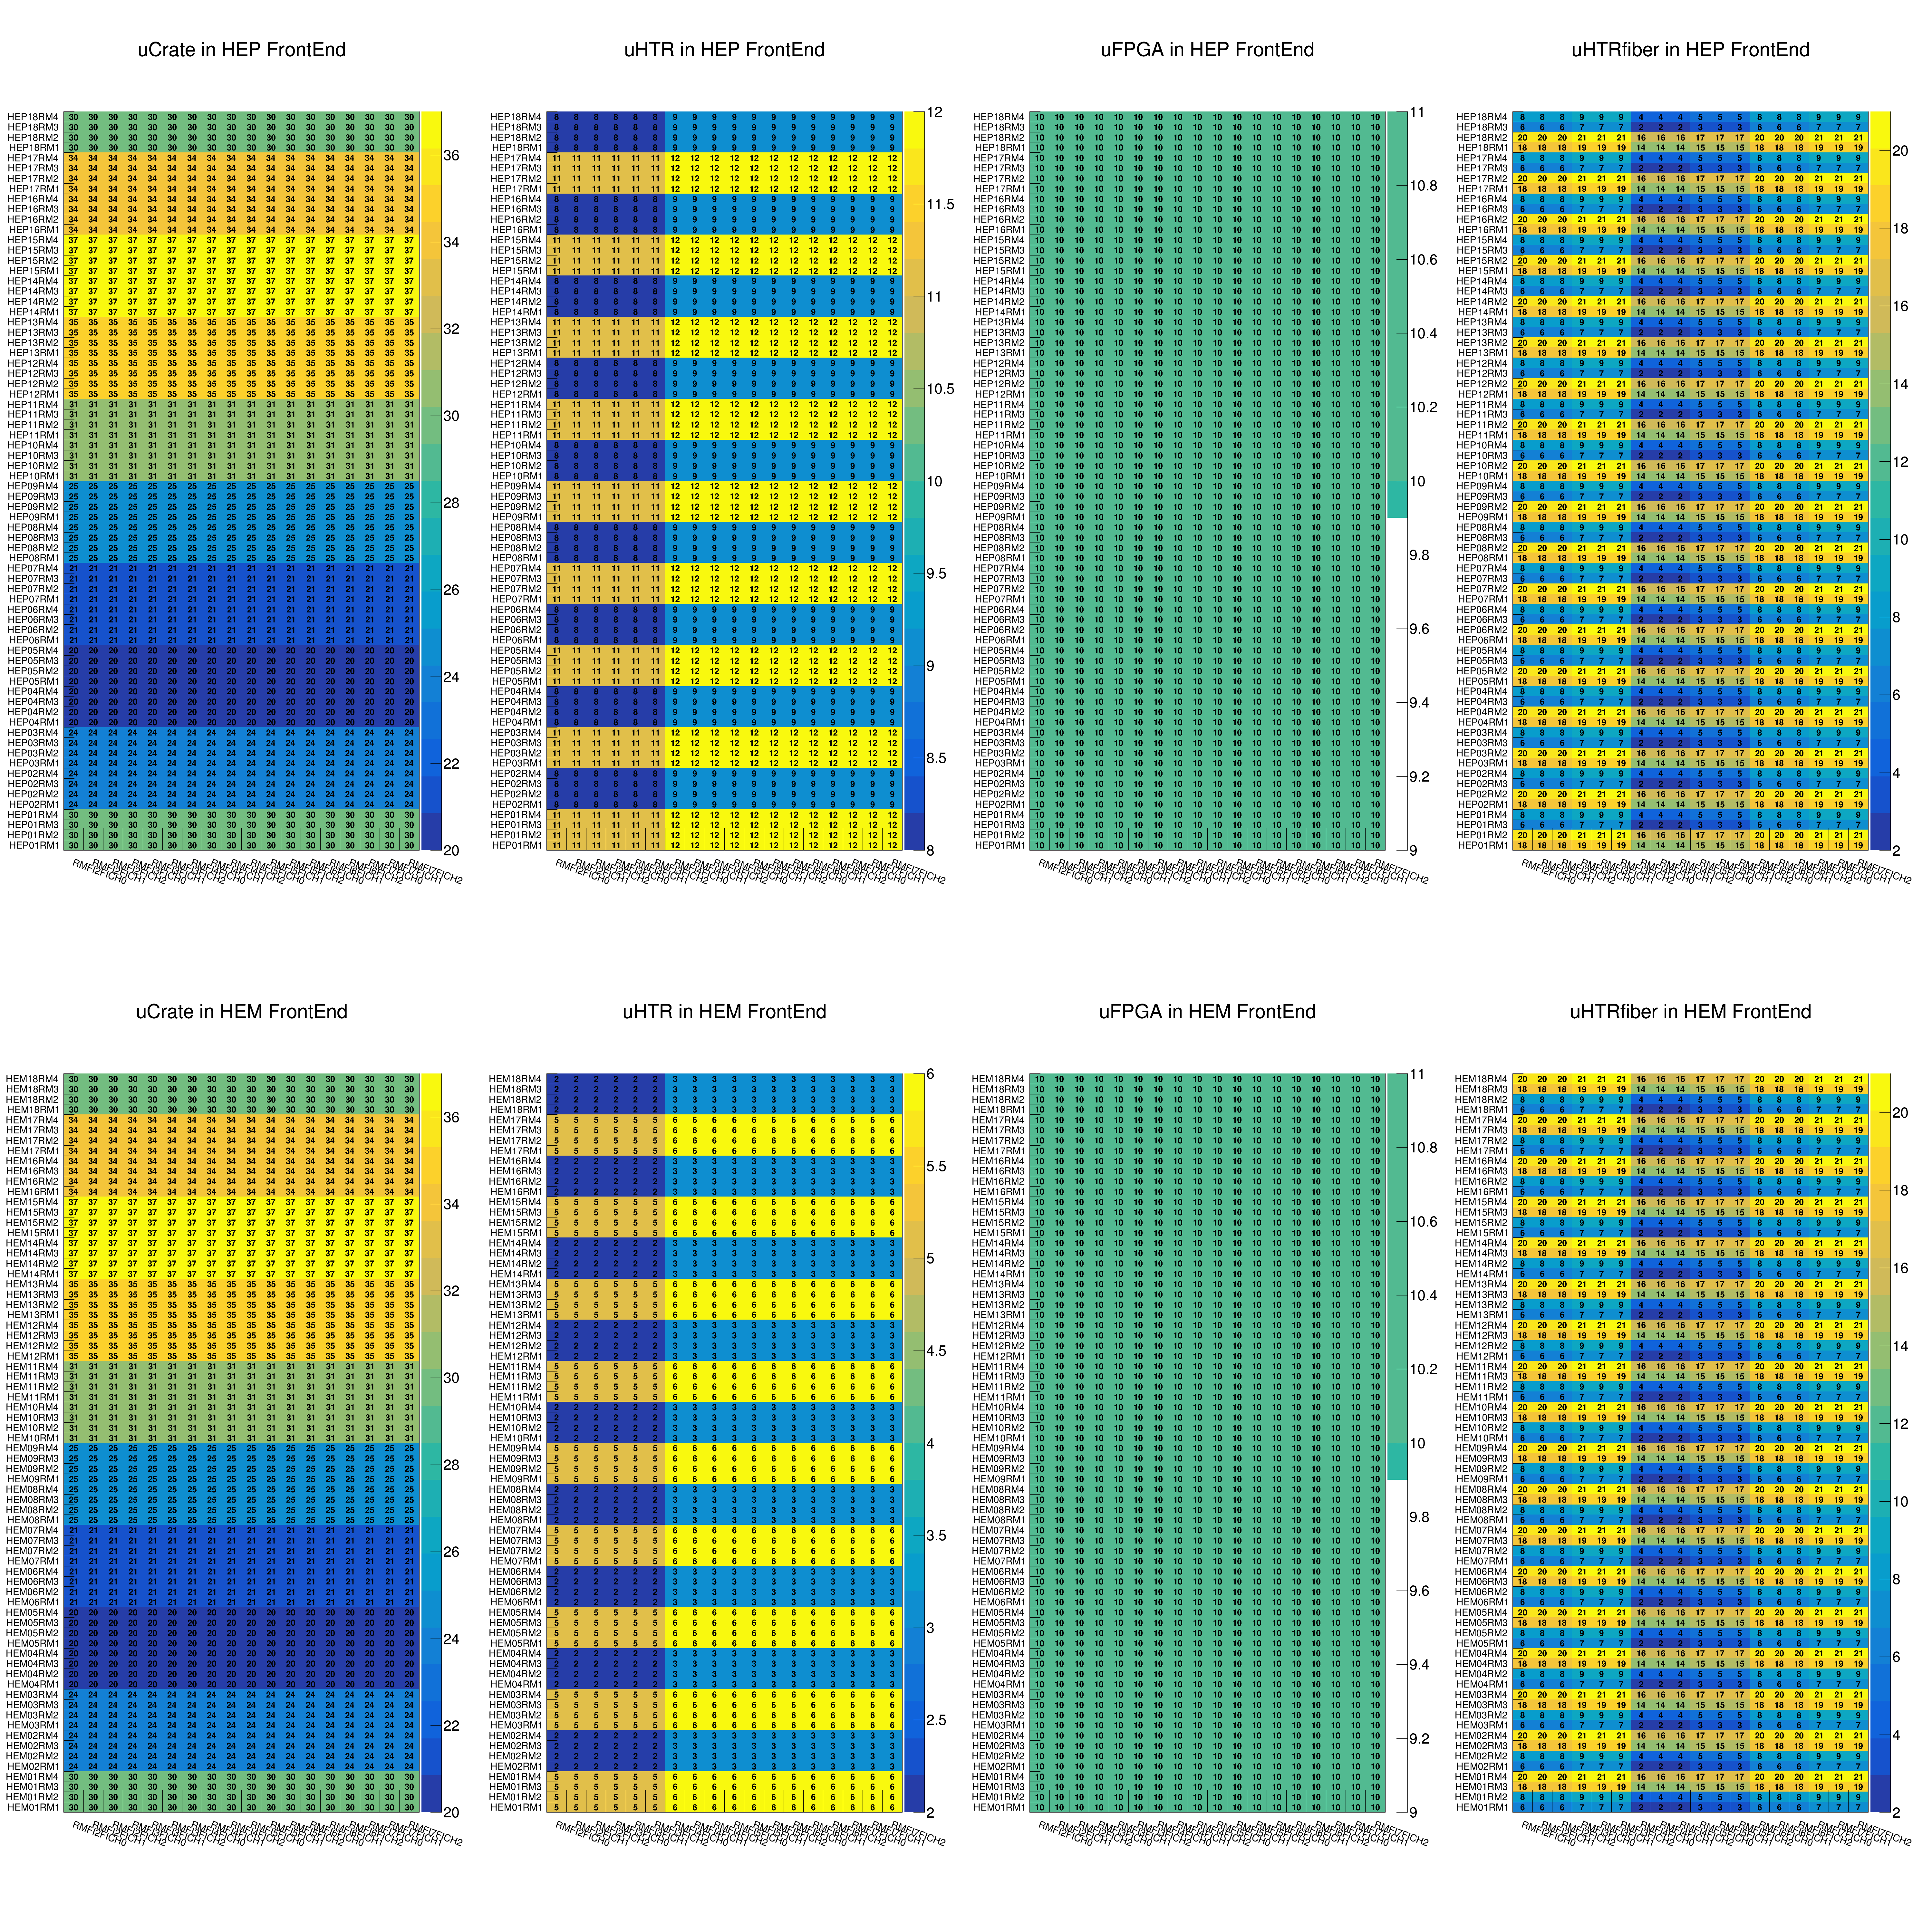
\includegraphics[width=0.8\textwidth]{figures/c3/c3_cms_hcalhelmapfebe.png}
 \end{center}
 \caption{Backend coordinates in Frontend coordinates, HCAL endcap phrase 1 backend plus phrase 0 frontend in 2016 operation}
 \label{fig:c3cmshcalhelmapfebe}
\end{figure}

\begin{figure}[htbp]
 \begin{center}
  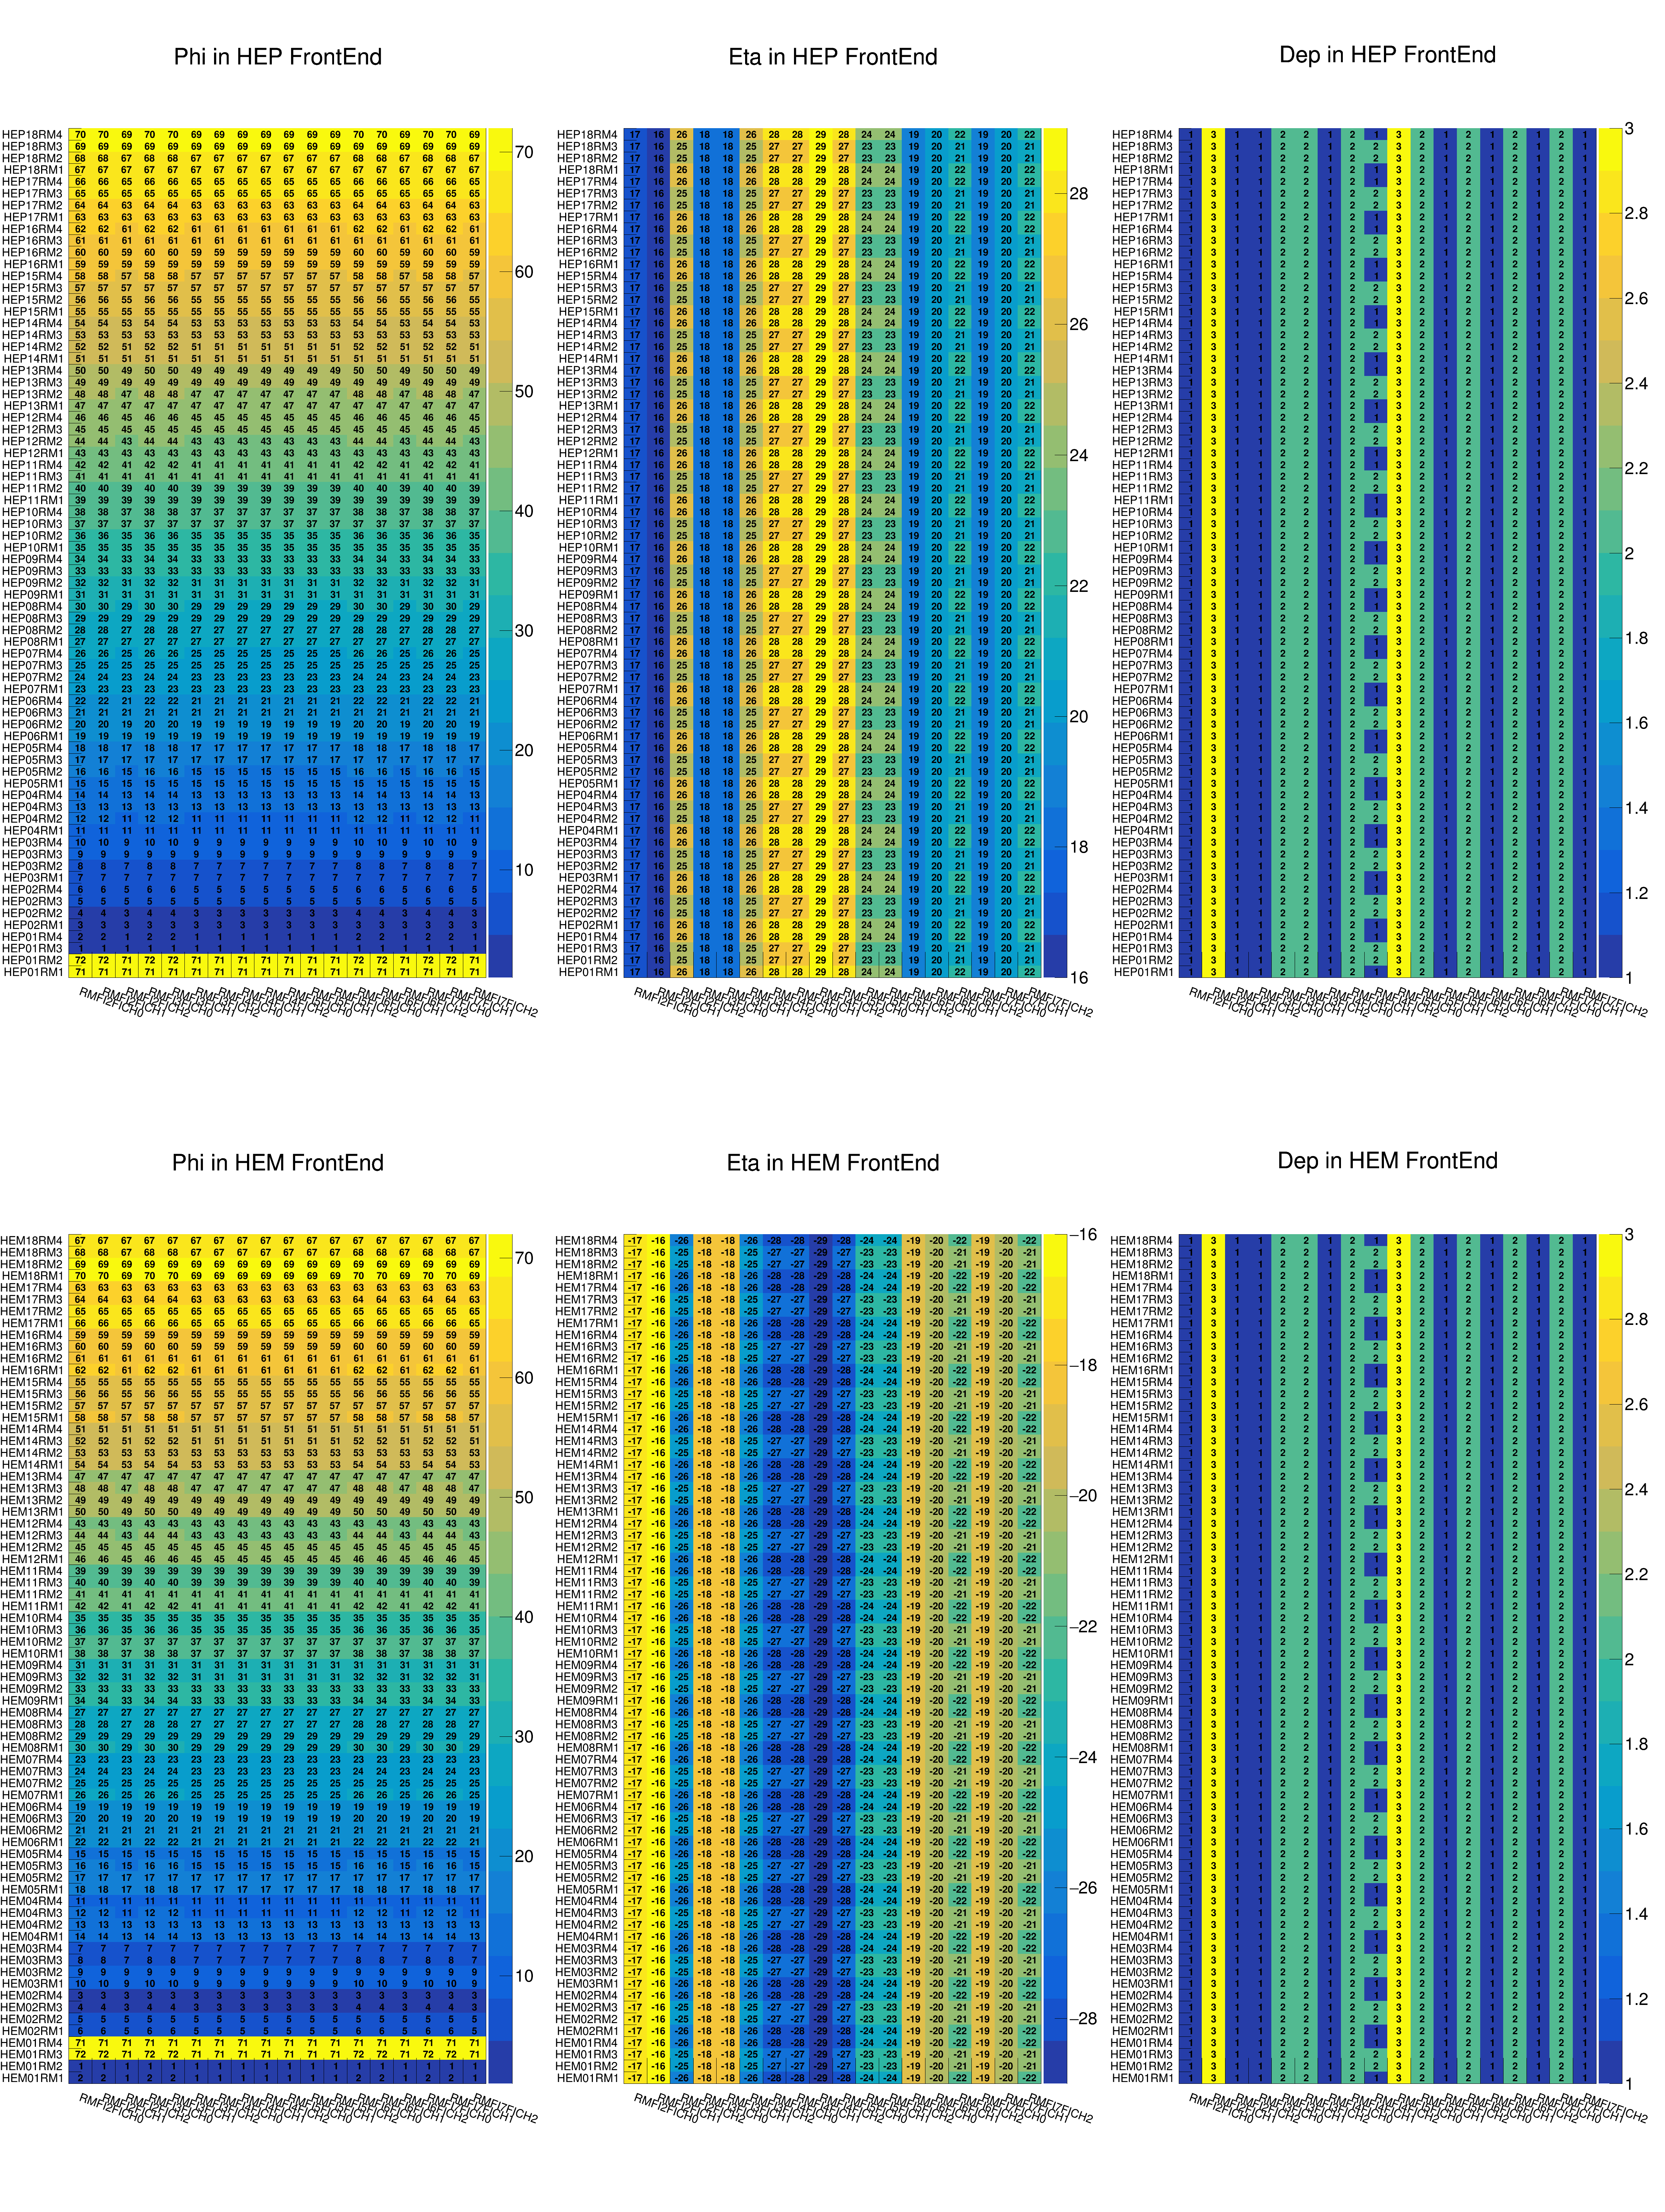
\includegraphics[width=0.8\textwidth]{figures/c3/c3_cms_hcalhelmapfegeo.png}
 \end{center}
 \caption{Detector coordinates in Frontend coordinates, HCAL endcap phrase 1 backend plus phrase 0 frontend in 2016 operation}
 \label{fig:c3cmshcalhelmapfegeo}
\end{figure}


The subset of the HCAL Logical map can be critical in the software world. One of the most important applications is the electronics map (EMap). The HCAL electronics map is a subset of logical map that contains backend coordinates and detector coordinates. As we mentioned, we the reconstruction software need to call for the EMap in the database to obtain the detector coordinates from backend coordinates. This is a necessary step in the RAW to DIGI in reconstruction and DIGI to RAW in MC simulation. Another application is the QIE calibration table. In the DIGI to RECO step, we need to translate from ADC (Analog Digital count) to the fC with the piecewise linear QIE gain function. This map is produced from logical map and pushed into database. The robustness of the Logical map is critical for the HCAL offline reconstruction. 

\subsubsection{Muon Detectors}

The importance of the Muon detectors is implied by the experiment’s middle name ("M" is CMS). The CMS muon detectors provide precise measurement of muon tracks with the support of strong magnet field (3.8T). The measurement of muons is useful in both standard model physics (e.g. Higgs to ZZ) and new physics search (e.g. leptonic channel supersymmetry). More over, the muon system also provide muon related trigger to reduce the data rate.

The CMS muon detectors consist of three sub-detectors: Drift tube in the barrel region, cathode strip chamber in the endcap and resistive plate chamber in both barrel and endcap. A layout of CMS muon detectors are showed in the Fig.~\ref{fig:c3cms2dmuondets}. More details are demonstrated in the following sections. 

\begin{figure}[htbp]
 \begin{center}
  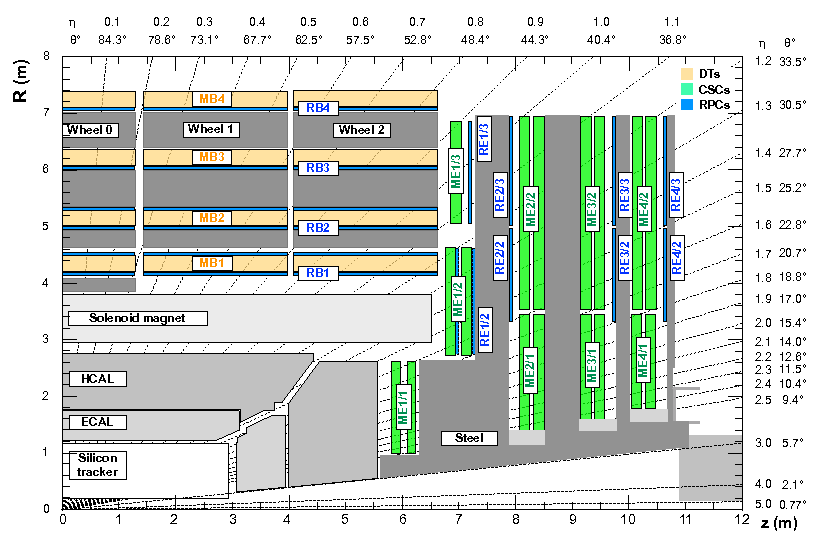
\includegraphics[width=0.8\textwidth]{figures/c3/c3_cms_2dmuondets.png}
 \end{center}
 \caption{Two dimensional CMS inner tracking system layout, phrase 0}
 \label{fig:c3cms2dmuondets}
\end{figure}

\paragraph{Drift Tubes}
Drift tubes (DT) are the part of CMS muon detectors that measure the muon tracks in the barrel region. The basic unit of the drift tubes is the drift cell. A drift cell is a 42mm-wide tube contains a thin conductive wire at high positive voltage within a gas volume. The muon knocks electron off the atom of the gas when it travel through the tube. The muon tracks can be reconstructed by measuring the drift time for different cells. 

Like the HCAL outer, the Drift tubes contain 5 wheels along the z-axis, 4 stations for each wheel, labeled as MB1, MB2, MB3 and MB4. The three inner stations have 60 drift chambers each and the outer chamber has 70. A drift chamber consists of 2 or 3 super layers, each made of by 4 layers of drift cells staggered by half of cell. This honeycomb geometry gives an excellent time-tagging capability, with a time resolution of a few nanoseconds. The full DT provides the pseudo-rapidity coverage $0<|\eta|<1.2$.

\paragraph{Cathode Strip Chambers}
Cathode strip chamber (CSC) is one of the CMS muon detectors that located in the endcap region. CSC is also a type of wire chamber, but different from the DT, CSC measures the location (to be specific, phi coordinates) instead of drift time. The CSC consists arrays of positively charged anode wires crossed with negatively charged copper cathode strip within a gas volume. The muon will knock the electron off from the gas atom. Then the electron will move to the anode wire to create an avalanche. Positive ions also move to the cathode and trigger a charged pulse.

The CMS endcap muon system consists of 468 cathode strip chambers in the following arrangement: 72 ME1/1, 72 ME1/2, 72 ME1/3, 36 ME2/1, 72 ME2/2, 36 ME3/1, 72 ME3/2, and 36 ME4/1. The full CSC provides the pseudo-rapidity coverage $1.2<|\eta|<2.4$. 

As we will mention at the beginning of next section, the RPC is designed as a fast response provider to trigger. However, for the endcap region, CSC is already good enough to satisfy the trigger requirement in the current instantaneous luminosity of the LHC. Moreover, CSC has a better spatial resolution and more pseudo-rapidity coverage, which provide a precise measurement for the endcap muons.

\paragraph{Resistive Plate Chambers}
Resistive plate chamber (RPC) is a fast gaseous detector that provides a muon trigger system in parallel with the DT and CSC. The RPC is a two high resistively plastic parallel plates system with gas in the middle. One of the plates is the positively charged anode and the other is negatively charged cathode. Like the CSC, the electron of gas will be knocked off when muon pass through, and then trigger avalanche. The pattern of hits on the cathodes will provide a quick measurement on the muon momentum and then pass to trigger for decision-making. In the CMS RPC, we are using the double-gap module instead of the single-gap one. This allows a lower bias voltage requirement of each single-gap and higher detector efficiency. The RPC performance is a combination of good spatial resolution and time resolution (one nanosecond). 

The CMS RPCs are distributed in both barrel and endcap region. There are 96 RPCs each wheel in barrel region. More details of the distribution are listed in the Table~\ref{tab:c3cmsrpc}. In the endcap region, we have 3 RPC stations in the phrase 0 design. In order to keep the high muon reconstruction efficiency with run2 condition, the fourth disk is installed during the long shutdown 1 for the phrase 1 upgrade. The full RPC have the same pseudo-rapidity coverage as DT in barrel, and smaller coverage ($1.2<|\eta|<2.1$) than CSC in endcap.

\begin{table}[htbp]
\fontsize{10 pt}{1.2 em}
\selectfont
\begin{centering}
\caption{\label{tab:c3cmsrpc} Numbers of RPCs for different wheels}
\hspace*{-4ex}
\begin{tabular}{|c|c|c|c|c|c|c|}
\hline
 RPC &  W+2 & W+1 & W0 & W-1 & W-2 & Total \\
\hline
 RB1(in) & 12 & 12 & 12 & 12 & 12 & 60 \\
\hline
 RB1(out) & 12 & 12 & 12 & 12 & 12 & 60 \\
\hline
 RB2/2(in) & 12 & - & - & - & 12 & 24 \\
\hline
 RB2/2(out) & - & 12 & 12 & 12 & - & 36 \\
\hline
 RB2/3(in) & - & 12 & 12 & 12 & - & 36 \\
\hline
 RB2/3(out) & 12 & - & - & - & 12 & 24 \\
\hline
 RB3 & 24 & 24 & 24 & 24 & 24 & 120 \\
\hline
 RB4 & 24 & 24 & 24 & 24 & 24 & 120 \\
\hline
 Total & 96 & 96 & 96 & 96 & 96 & 480 \\
\hline
\end{tabular}
\par\end{centering}
\end{table}

\subsubsection{Trigger system}

The LHC have bunch crossing in every 25 ns, which means 40MHz in data rate. It is impossible for the data acquisition and storage system to deal with all of them. And it is not necessary too, since not all the events are interested in the physics analysis. Therefore, we need a system to reduce the data rate and select the events that we are interested in. The system is called trigger system - - - only triggered data will be read and stored from the LHC collision. 

The CMS trigger system is a 2-level trigger system: the FPGA based L1T (Level 1 trigger) and PCs farm based HLT (High level trigger). In the old days we always add a custom hardware L2T layer in between L1T and HLT to ease the computing speed gap. However, with improvement of PCs farm’s computing power, we can avoid the additional L2T. This gives us a more robust system with less complicate structure. 

The CMS L1T system receives part of the information from sub detectors and has a rough estimation on the physics object in the FPGA level. The data rate is reduced from 40MHz to 100kHz (85kHz to 90kHZ in real operation, mainly limited by data acquisition system) after the L1T. CMS L1T has been upgraded (Phrase 1) during the 2015-2016 YETS and 2016-2017 EYETS since the beam intensity increase significantly in the LHC run 2. The new scheme plot of phrase 1 L1T is showed in the Fig.~\ref{fig:c3cmsl1scheme}. The calorimeters will send the trigger primitive to the calo trigger layer then finally go to global trigger. And muon system will send information to the global muon trigger then finally arrive at global trigger. Then the L1A (level 1 acceptance) will be generated and sent to the sub detectors through TCDS (timing, control and distribution system). The sub detectors will send the information to data acquisition or keep on taking data for next bunch crossing based on the L1 decision. 

\begin{figure}[htbp]
 \begin{center}
  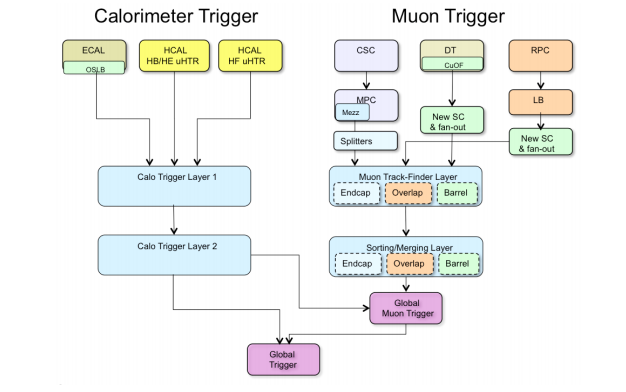
\includegraphics[width=0.8\textwidth]{figures/c3/c3_cms_l1scheme.png}
 \end{center}
 \caption{Dataflow for the overall phrase 1 trigger system}
 \label{fig:c3cmsl1scheme}
\end{figure}

The CMS HLT system uses all the information from detector readout and applies a simplified algorithm to reconstruct physics object. The promptly reconstructed object will be applied in the different high-level trigger menu for different physics purpose. However, just like the L1T, we have bandwidth limit for the HLT also. The current data rate after the HLT are constraint to be around 1000 Hz which is limited mainly by offline storage rather than online computing. HLT is the interface between physics analysis and online operation. On one side, each physics analysis group will have a trigger contact to collect the desired trigger menu from analyzers and make a proposal of a full menu set with rate estimation to the HLT that satisfy the data rate limit. On the other side, each the HLT menu will take at least one L1 seed as a starting point of the high-level trigger.

The current (Phrase 1) trigger system will be continue in operation until the end of LHC run 3. However, there is a huge challenge on the trigger system with the following HL-LHC. Track trigger is necessary to maintain the current physics acceptance with the L1 rate around 1MHz. 

\subsection{Event Reconstrunction}

The data from the central data acquisition system will be selected and built in the high-level trigger farm and then transferred to the primary computing grid at CERN (Tier-0). The data directly from the detector electronics is called DAQ-RAW, which is the input of the online HLT cluster. The data will be reformatted and filtered with high-level trigger in the cluster. The outcome data is called RAW. Comparing to the DAQ-RAW, the RAW contains the HLT information and ready for offline reconstruction after reformatting. 

Before entering the offline reconstruction chain, the data stream is filtered into different primary datasets (PD) for various purposes. Most of the categories are based on physics analysis and level 1 trigger. For example, in the all-hadronic SUSY search, the common PD for search region is HTMHT or MET. For the control region, we can select SingleElectron or SingleMuon PD. Then, the RAW with different PD streams will be delivered into the offline reconstruction system (CERN Tier-0 or any Tier-1, Fig.~\ref{fig:c3cmstiers}). 

\begin{figure}[htbp]
 \begin{center}
  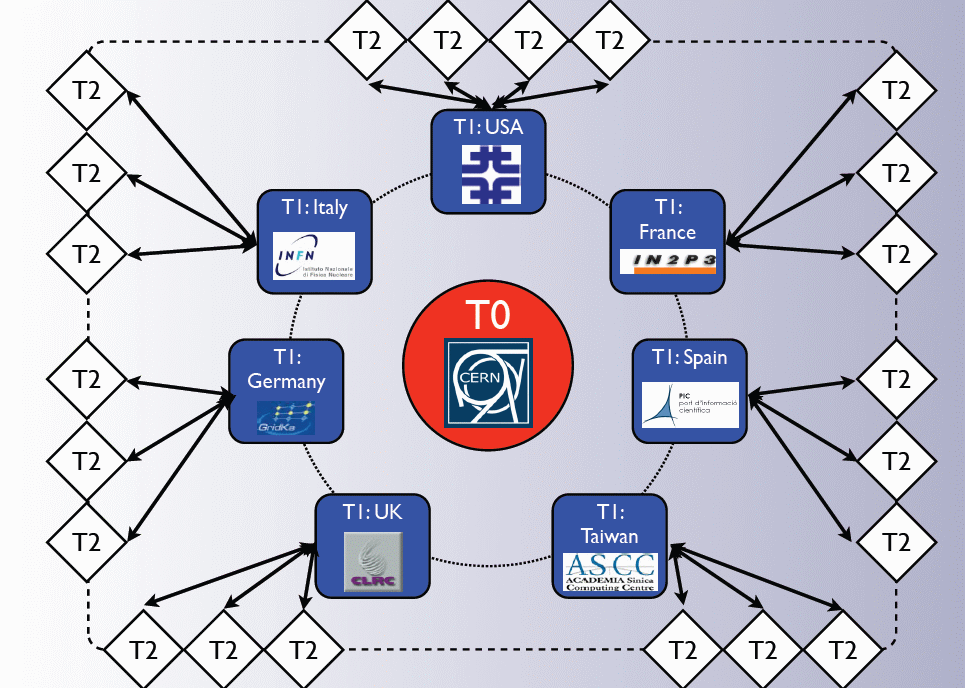
\includegraphics[width=0.8\textwidth]{figures/c3/c3_cms_tiers.png}
 \end{center}
 \caption{CMS offline computing structure}
 \label{fig:c3cmstiers}
\end{figure}

In the offline reconstruction, the RAW dataset will be unpacked from the electronics based digital counts to detector based digital hits. This is so called RAW to DIGI step in the reconstruction. After that, the DIGI will be converted to reconstructed hits with calibration information. This is called DIGI to RecHits step. The offline database are highly involved in these 2 steps, providing electronic-detector map, calibration table, pedestal subtraction, radiation damage correction, etc. Then, the physics objects will be generated with the reconstructed algorithm. The outcome dataset after the offline reconstruction is called RECO, which combines the RecHits and physics object information together. 

However, the size of the RECO dataset is about 1.3 MB per event. The further reduce of the data size is necessary for the physics analysis. Therefore, the information that not very commonly used for physics analysis is dropped to form a new data format: miniAOD. It contains the standard physics objects that used by most of the CMS physics analysis group. More details of those objects will be discussed in the following sections. 

\subsubsection{Tracks}

Tracks are detected by inner silicon detector signals in the CMS to form the basis of the event reconstruction. Track reconstruction serves the following purposes: 
\begin{itemize}
\item Vertex reconstruction: The vertexes in the proton-proton collision can be reconstructed from the gather point of tracks. However, there can be multiple vertexes in one event because the pile up effect. The vertex with the maximum sum of the square of the $p_{T}$ of all the associated tracks is identified as the primary vertex. We can also reconstruct the secondary vertex from the primary one. The secondary vertex information is useful in the b-jet identification.
\item Momentum measurement: The CMS inner silicon system has a high resolution in the track momentum measurement because of the strong magnetic field (3.8T). The jet $p_{T}$ measurement benefits a lot from the high precision track momentum with the particle flow algorithm. More details will be covered in the jet reconstruction section.
\item Particle identification: The charged can be identified with track information. For example, an electron candidate is found when the energy deposit in ECAL supercluster can be associated with track. Muon identification can also benefits from the inner track matching technique.
\end{itemize}

Given the importance of track reconstruction in physics, a reliable algorithm is required. The desirable algorithm must have a near 100\% efficiency in track reconstruction together with relatively small fake rate. The jet energy can be deadly mis-measured with an unidentified or fake track.
There are two steps in the track reconstruction: 
\begin{itemize}
\item Local reconstruction: the signals from the strip and pixel are clustered to evaluate the position and error matrices of hits.
\item Global reconstruction: Tracks are reconstructed with several iteration of the combinatorial track finder method\cite{Adam:2005cg}. Different seed will be used in different iteration to improve the tracking efficiency for various types of tracks.
\end{itemize}
The track finder algorithm is very powerful. It can even find the track with very low energy ($p_{T}<2 GeV$). Some of the low energy tracks have more number of hits than the number of detector layers, others tracks cannot reach to the preshower. Those tracks are kept in the data file for the low energy physics study at CMS. 

\subsubsection{Electrons}
The electron reconstruction in CMS relies on the information from inner tracker and ECAL. The track momentum can be measured with smaller uncertainty in the inner tracker system. On the opposite, the calorimeter has a better resolution for the high-energy object. Therefore, a mixture of "ECAL seed" and "tracker seed" algorithm is designed to optimize the electron identification in both high and low $p_{T}$ spectrum. 

The ECAL seed electron identification algorithm starts from the supercluster energy deposit in the ECAL. The supercluster is a 5 by 5 cluster combo in the ECAL. The initial energy and position in the supercluster will be used to estimate the electron trajectory in the first tracker layer. On the opposite, the tracker-based method begins with the tracks that are reconstructed by the general algorithm for charged particles. The tracks will be sent to a pre-selection and then matched to the ECAL supercluster. This mixture seed method has been validated with electron from W boson decay in 2010\cite{Khachatryan:2015hwa}. 

The electron identification group also provides several working points to satisfy the needs from various physics analysis. For example, we choose the "Veto" working point in the SUSY analysis described in this thesis. The "Veto" has the loosest identification criteria, which help us to reject leptonic decayed background to the most extent. 
\subsubsection{Jets and Particle Flow}

\subsubsection{Missing Transverse Energy}

\subsubsection{Muons}
The muon is a heavy particle that can penetrate the calorimeter and detector by the muon system outside the solenoid. The muon reconstruction has two traditional approaches: 

\begin{itemize}
	\item Global Muon reconstruction: The muon tracks are reconstructed first inside the muon system (DT, RPC, CSC) by a standalone method. Then, the muon standalone muon track will be matched with a tracker track by comparing the parameters of the two tracks. Finally, a global muon track will be derived from the hits of the two tracks by Kalman-filter method\cite{Fruhwirth:1987fm}. This is so called outside-in method since we start from the muon system, which is outer member of the CMS detectors. 
\item Tracker Muon reconstruction: In this approach, we start from the tracks reconstructed by the inner silicon detectors. The tracks with $p_{T}<0.5 GeV$ and momentum $p>2.5GeV$ will be selected as the potential muon candidate. Then, the track will be extrapolated to the muon system considering the magnet field, average expected energy loss and multiple coulomb scattering effects. The track will be qualified as muon track if at least one muon hit matched with this track. This is inside-out method since it begins with the inner tracker system. 
\end{itemize}

The global muon reconstruction method has a better momentum resolution in the hard muons. The reason is the high $p_{T}$ tracker tracks performance is limited by the small geometry of the inner tracker system. However, the tracker muon reconstruction method has a better performance in the soft muons. This originates from the excellent low $p_{T}$ tracks measurement of inner tracker system. 

A particle flow based algorithm has been designed to obtain good performance for both soft and hard muons. This particle flow muon reconstruction method is a combination of outside-in and inside-out methods. In this approach, global muon tracks and tracker tracks are gathered together and then selected with special criteria. The selection criteria are adjusted depending on environment of muon (e.g. isolation) and other detector input (e.g. energy deposit in calorimeter). This method is optimized to identify the muons within jets. The performances of the three approaches have been studied in\cite{Chatrchyan:2012xi}. 
